%%%%%%%%%%%%%%%%%%%%%%%%%%%%%%%
%% Folie: Architecture  %%
%%%%%%%%%%%%%%%%%%%%%%%%%%%%%%%
\begin{frame}
    \frametitle{Architecture}

U-Net derivative proposed in the paper: \\[\baselineskip]

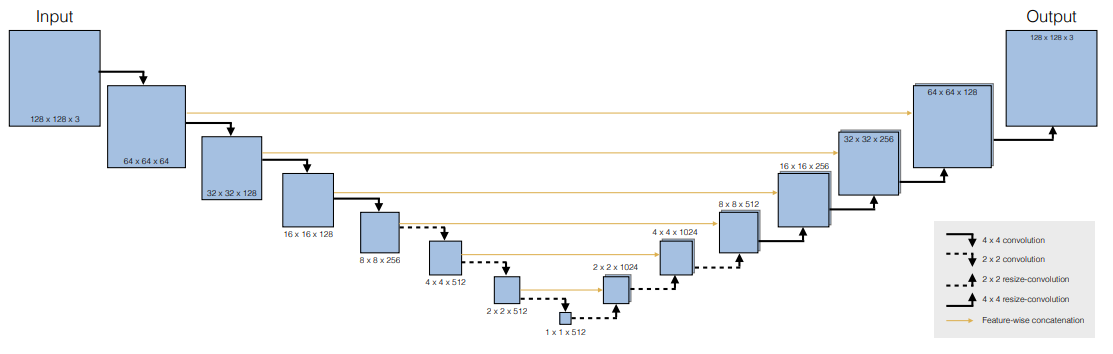
\includegraphics[width=\textwidth, height=.55\textheight]{./Ressourcen/Praesentation/Bilder/architecture.png}%
\newline
Taken from \url{https://arxiv.org/pdf/1810.08217.pdf}
\end{frame}
\clearpage

\begin{frame}
    \frametitle{Architecture -- Convolutional blocks}
\vspace*{0.8cm}
\begin{multicols}{2}
    \textbf{Encoder}

    1. Activation -- Leaky ReLu (0.2)

    2. Convolution -- Width down, Depth up

    3. Batch normalization

    4. Dropout (1\%)
    \vfill\columnbreak
    \textbf{Decoder}
    
    1. Activation -- ReLu
    
    2. Upsampling -- linear (2.0)

    3. Convolution -- Width up, Depth down

    4. Batch normalization

    5. Dropout (1\%)
    
\end{multicols}
    
\end{frame}
\clearpage

\begin{frame}
    \frametitle{Architecture -- Evaluation}
Error percentage of different activation functions after 160k iterations (266 epochs).\newline
PReLu achieves the best error rates (p, vel, combined: \textbf{14.69}\%, \textbf{2.216}\%, \textbf{2.676}\% -- Default: 14.76\%, 2.296\%, 2.787\%)\newline
\begin{center}
	\vspace*{-1.2cm}
    \begin{tikzpicture}
        \begin{axis}[
                ybar=10,
                bar width=27.1,
                axis line style={transparent},
                every tick/.style={transparent},
                enlarge x limits=0.145, % X-Achse skalieren
                clip limits=true,
                ymin=0,
                ymax=22.5,
                width=\textwidth,
                height=.65\textheight,
                symbolic x coords={Default,PReLu,ReLu},
                xticklabels={Default,PReLu,ReLu},
                xtick=data,
                ytick={0,5,10,15,20},
                %ytick={0,3,6,9,12,15,18,21,24,27,30},
                every tick label/.append style={font=\fontsize{13}{14}\selectfont},
                ymajorgrids,
                legend image code/.code={\draw[draw=none] (0cm,-0.12cm) rectangle (0.29cm,0.17cm);}, % Legenden-Symbol  
                legend columns=3,
                reverse legend,
                legend style={
                    font={\usebeamerfont{footnote}},
                    fill=none,
                    draw=none,
                    /tikz/every odd column/.append style={column sep=0.07cm}, % Abstand zwischen Legenden-Symbol
                    /tikz/every even column/.append style={column sep=0.8cm} % Abstand zwischen den Legendeneinträgen
                 },
                legend to name=PraesentationDiagrammVertikalLegende
            ]
            
            \addlegendentry{Combined}        
            \addlegendentry{Pressure}    
            \addlegendentry{Velocity}    
            
            %comb
            \addplot[color=TUMBlauDunkel, fill=TUMBlauDunkel] coordinates {
                (Default,2.78)
                (PReLu,2.67)
                (ReLu,3.17)
            };
            
            %p
            \addplot[color=TUMBlauHell, fill=TUMBlauHell] coordinates {
                (Default,14.76)
                (PReLu,14.69)
                (ReLu,39.39)
            };
            
            %v
            \addplot[color=TUMBlauMittel, fill=TUMBlauMittel] coordinates {
                (Default,2.29)
                (PReLu,2.21)
                (ReLu,2.97)
            };        
        \end{axis}
    \end{tikzpicture}

    \vspace*{-8mm}
    \ref*{PraesentationDiagrammVertikalLegende}%
\end{center}
\end{frame}
\clearpage

\begin{frame}
    \frametitle{Architecture -- Evaluation}
    \vspace*{.1cm}
\begin{multicols}{2}
	Training loss (Default: b, PReLu: r, ReLu: g)
	
	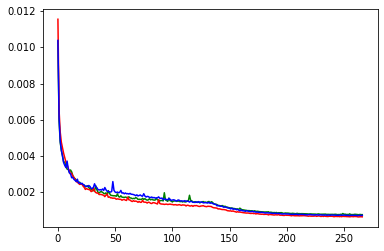
\includegraphics[width=.9\columnwidth, height=.6\textheight]{./Ressourcen/Praesentation/Bilder/train_loss.png}%
    \vfill\columnbreak
    Validation loss (Default: b, PReLu: r, ReLu: g)
    
    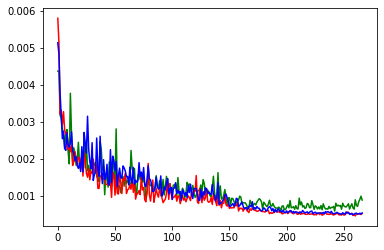
\includegraphics[width=.9\columnwidth, height=.6\textheight]{./Ressourcen/Praesentation/Bilder/val_loss.png}%
\end{multicols}
    
\end{frame}
\clearpage